\section{Experiments}
\label{sec:experiments}

We evaluate \name by separating the two context-curation strategies it
introduces. The iteration-level strategy bounds and labels the history
seen by the proposer, replacing unstructured full-history browsing with
directed historical attention. The file-level strategy can be composed
with it to reallocate the proposer's bounded inspection budget toward
files with observed utility. These strategies are not independent
additive modules, nor are both required in every setting. They are
alternative and composable ways to route the same fixed-inspection
bottleneck.

\subsection{Setup}
\label{sec:setup}
\textbf{Benchmarks.}
We evaluate \name on three benchmarks chosen to span the two
failure modes our strategies address: \emph{redundant iteration
history} (long propose--evaluate traces with stale or failed
attempts) and \emph{redundant file context} (large workspaces with
many irrelevant files).
\begin{itemize}[leftmargin=*,topsep=0pt]
    \item \textbf{LoCoMo}~\cite{maharana2024locomo} is a
    multi-session long-conversation benchmark whose inner harness
    is a conversational memory system. The harness has many
    specialised components that benefit from many refinement
    rounds, making it our main testbed for joint iteration--file
    curation. We optimise on 80 training examples and report held-out
    test results on the full 1,449-example split.
    \item \textbf{LongMemEval}~\cite{wu2024longmemeval} is a
    long-term memory benchmark whose inner harness is a
    memory-augmented assistant tested on retrieval, temporal
    reasoning, and consolidation across long histories. We optimise on
    100 training examples and report held-out test results on the
    400-example test split.
    \item \textbf{SWE-bench Verified}~\cite{openai2024swebenchverified}
    is a human-curated subset of 500 GitHub issues from 12 Python
    repositories. We optimise on the \texttt{trainfirst30} pool
    and re-evaluate selected candidates on the full 500-issue verified
    set. SWE-bench Verified tests whether curation gains transfer to
    multi-file coding-agent harnesses.
\end{itemize}

\textbf{Inner-harness solvers.}
On the memory benchmarks the inner harness is the MemGPT-style
memory agent~\cite{packer2023memgpt} optimised by the proposer.
On SWE-bench the inner-harness candidates are evaluated by a fixed
Mini-SWE agent driven by DeepSeek~v4 Flash; this isolates
harness-curation effects from inner-solver variance.

\textbf{Proposer families.}
We instantiate the meta-agent on top of two coding-agent scaffolds:
a Codex CLI proposer with GPT-5.4 as the backbone, and a Claude
Code-compatible proposer with Kimi~K2.6 as the backbone. We refer to
these as \emph{codex54} and \emph{claudekimi}. Both run on the memory
benchmarks; SWE-bench is run with claudekimi only.

\textbf{Baseline.}
The single end-to-end baseline is \textbf{Full-context}, the
default Meta-Harness configuration~\cite{lee2026metaharness}: every
iteration uses the full revision history and an unrestricted file
tree, with no best/worst labelling. We aggregate two variants
(\texttt{default} and \texttt{default+direction}) into a single
\emph{default-family} cell because both fix the budget at
\texttt{high} by construction.

\textbf{Optimisation protocol and reporting conventions.}
Each run executes 30 propose--evaluate iterations on the training
split. We retain the candidate frontier under a passrate-priority
Pareto rule with quality gap $\delta\!=\!0.125$. Each
(benchmark, proposer, policy) cell is run multiple times for
numerical stability. Within each cell we report two complementary
statistics: \emph{test mean$\pm$std} aggregates all retained runs,
and \emph{best test} reports the highest held-out passrate of any
retained run. Per-propose token cost columns are taken from the
single best-by-test run in each cell, since cost is reported on the
representative run for that cell.
Token cost is reported in millions of tokens per propose
(\texttt{total/prop}, including cache reads) summed over input,
output, and cache-read tokens. Figures use the same single
best-by-test run per cell to avoid mixing replicates of the same
experiment into one curve.

\subsection{Iteration-axis curation improves search quality}
\label{sec:iter_axis}

We first isolate the \emph{iteration-axis} strategy's contribution
before any file-level utility model is in play. The \emph{Progressive} policy of
Section~\ref{ssec:iteration} surfaces best/worst-tagged ref-iter
directories under a \texttt{low}$\,\to\,$\texttt{medium}$\,\to\,$\texttt{high}
budget state machine but does \emph{not} curate which files within
those directories the proposer sees. Comparing Progressive against
the default-family baseline isolates the iter-axis contribution from
the file-axis contribution: the only new signal is which historical
iterations are exposed and how they are labelled.

Table~\ref{tab:main} reports the cost--quality trade-off across all
five (benchmark, proposer) cells, including the SWE-bench full
verified-set evaluation. Rows are stacked by curation depth:
\emph{default},
\emph{Progressive} (iter axis only), and \emph{\name} (iter+file,
discussed in Section~\ref{sec:file_axis}). Figure~\ref{fig:pareto}
plots the four memory cells in cost--quality space.

\begin{table}[t]
\centering
\small
\caption{Cost--quality across all (benchmark, proposer) cells.
Rows are stacked by curation depth. \emph{Test mean$\pm$std}
averages all retained runs in the cell; \emph{best test} is the
highest held-out passrate of any retained run; per-propose cost
columns are reported on that best-by-test run. The $\Delta$ column
reports total/propose savings relative to the cell's default row.
SWE-bench numbers are train-pool train passrate and full-500 verified
passrate; $\Delta$ verified is the gain on the full verified set.}
\label{tab:main}
\begin{tabular}{@{}llrrrr@{}}
\toprule
Benchmark & Policy & test mean$\pm$std & best test & total/prop & $\Delta$ \\
\midrule
\multicolumn{6}{l}{\textit{LoCoMo / claudekimi}} \\
 & default-family       & $0.331 \pm 0.015$ & $0.342$ & $3.42$M & --- \\
 & Progressive (iter)   & $0.355 \pm 0.021$ & $\mathbf{0.373}$ & $\mathbf{1.86}$\textbf{M} & $\mathbf{-46\%}$ \\
 & \name (iter+file)    & $\mathbf{0.355 \pm 0.008}$ & $0.362$ & $2.63$M & $-23\%$ \\
\midrule
\multicolumn{6}{l}{\textit{LoCoMo / codex54}} \\
 & default-family       & $0.331 \pm 0.013$ & $0.340$ & $3.42$M & --- \\
 & Progressive (iter)   & $\mathbf{0.374 \pm 0.014}$ & $\mathbf{0.388}$ & $2.46$M & $-28\%$ \\
 & \name (iter+file)    & $0.355 \pm 0.027$ & $0.387$ & $\mathbf{2.14}$\textbf{M} & $\mathbf{-37\%}$ \\
\midrule
\multicolumn{6}{l}{\textit{LongMemEval / claudekimi}} \\
 & default-family       & $0.498 \pm 0.030$ & $0.530$ & $3.71$M & --- \\
 & Progressive (iter)   & $0.505 \pm 0.013$ & $0.520$ & $3.37$M & $-9\%$ \\
 & \name (iter+file)    & $\mathbf{0.510 \pm 0.038}$ & $\mathbf{0.545}$ & $\mathbf{2.55}$\textbf{M} & $\mathbf{-31\%}$ \\
\midrule
\multicolumn{6}{l}{\textit{LongMemEval / codex54}} \\
 & default-family       & $0.497 \pm 0.010$ & $0.508$ & $2.93$M & --- \\
 & Progressive (iter)   & $\mathbf{0.499 \pm 0.028}$ & $\mathbf{0.528}$ & $2.66$M & $-9\%$ \\
 & \name (iter+file)    & $0.463 \pm 0.010$ & $0.473$ & $\mathbf{2.18}$\textbf{M} & $\mathbf{-26\%}$ \\
\midrule
\multicolumn{6}{l}{\textit{SWE-bench Verified / claudekimi (trainfirst30 $\to$ full500)}} \\
 & default-family       & train $0.500$ & verified $0.458$ & $3.22$M & --- \\
 & Progressive (iter)   & train $0.533$ & verified $0.620$ & $3.78$M & $+16.2$\,pp \\
 & \name (iter+file)    & train $0.533$ & verified $\mathbf{0.640}$ & $3.51$M & $\mathbf{+18.2}$\,\textbf{pp} \\
\bottomrule
\end{tabular}
\end{table}

\begin{figure}[t]
  \centering
  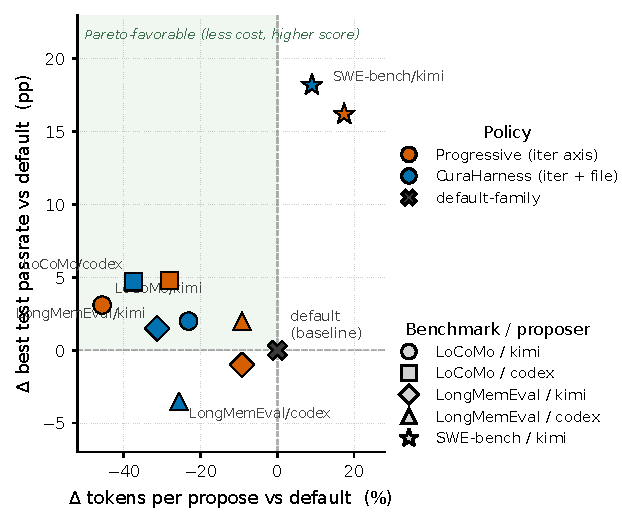
\includegraphics[width=\linewidth]{figures/pareto_cost_quality.pdf}
  \vspace{-6pt}
  \caption{Cost--quality positioning on the four memory cells.
  Each cell shows the single best-by-test retained run for default
  ($\blacksquare$), Progressive ($\bullet$, iter axis only), and
  \name ($\blacktriangle$, iter+file). Upper-left is the favourable
  region (less cost, higher score). Progressive improves mean test
  over default in all four memory cells; \name strictly dominates
  default in three cells and occupies a new cost-frontier point
  ($-26\%$ cost, $-3.4$\,pp test) on LongMemEval / codex54.}
  \label{fig:pareto}
\end{figure}

\textbf{Progressive improves mean held-out performance.}
Progressive's mean test passrate exceeds default-family in all four
memory cells: $+2.3$\,pp on LoCoMo claudekimi
($0.331 \!\to\! 0.355$), $+4.3$\,pp on LoCoMo codex54
($0.331 \!\to\! 0.374$), $+0.7$\,pp on LongMemEval claudekimi
($0.498 \!\to\! 0.505$), and $+0.25$\,pp on LongMemEval codex54
($0.497 \!\to\! 0.499$). The two LoCoMo gains sit at $1.5\sigma$
and $3.2\sigma$ above the default-family std and are clear of run
noise; the two LongMemEval gains lie within run std and should be
read as directional. In these cells, curating which prior iterations
the proposer attends to is enough to lift mean test even without a
file-side utility model.

\textbf{The effect extends to a coding-agent harness.}
On SWE-bench Verified, Progressive's trainfirst30 train passrate
($0.533$) is only $3.3$\,pp above default ($0.500$), but the
full-500 verified passrate jumps from $0.458$ to $0.620$
($+16.2$\,pp). The trainfirst30 pool compresses all policies into
a narrow $0.50$--$0.53$ band, which masks the mechanism difference
between full-context and curated context; the difference surfaces
on the larger verified set. The iter-axis mechanism is
not memory-benchmark-specific.

\textbf{Cost is a secondary, variable effect of iteration curation.}
Progressive's cost saving ranges from $-46\%$ on LoCoMo claudekimi
down to $-9\%$ on LongMemEval codex54, and rises to a $+17\%$
\emph{increase} on SWE-bench. Iteration curation is therefore not
primarily a token-reduction mechanism: it saves cost when labelled
history substitutes for proposer-side localisation, but the proposer
can also spend the narrower historical context on additional source
inspection or tool use.

\subsection{File-axis curation improves the cost--quality operating point}
\label{sec:file_axis}

We now layer the \emph{file-axis} bandit (Section~\ref{sec:bandit})
on top of Progressive's iter-axis state machine, yielding
\name. The bandit assigns delayed credit to files read by the
proposer and concentrates future attention on a UCB-scored hot pool;
this changes where the proposer spends its fixed read budget rather
than merely shrinking the workspace. Comparing \name against default
and Progressive therefore tests whether a file-utility prior improves
the cost--quality operating point under bounded historical exposure.

\textbf{File-axis curation gives a more stable cost-axis lever under
bounded historical exposure.}
Across all four memory cells \name reduces per-propose tokens by
$-23\%$ to $-37\%$ relative to default (Table~\ref{tab:main}), and is
the cheapest of the three policies in three of the four cells. This
pattern is more stable than Progressive's wider cost range
($-46\%$ to $-9\%$ on memory, with an increase on SWE-bench), but it
is conditional on the iteration-level scope. The file-axis prior pays
off when the iteration strategy has already bounded the historical
channel. If the full iteration history remains open, the bandit can add
policy metadata and hot-file guidance on top of an already large
context; in that setting it may redirect attention without reducing
total token volume.

\textbf{The lower-cost operating point comes with a cell-conditional
test trade-off.}
On three of the four memory cells \name strictly dominates default
on the cost-quality plane: $+2.4$\,pp at $-23\%$ cost on LoCoMo
claudekimi, $+2.5$\,pp at $-37\%$ on LoCoMo codex54, and
$+1.2$\,pp at $-31\%$ on LongMemEval claudekimi. The fourth cell,
LongMemEval codex54, scores $0.4625$ vs default $0.4967$
($-3.4$\,pp test) at $-26\%$ token cost. \name therefore introduces a
$2.18$M operating point within $3$--$4$\,pp of default, whereas the
default-family cell operates at $2.93$M total/propose. This is Pareto
frontier expansion rather than universal dominance: the file axis
creates lower-cost operating points at comparable quality in most
cells, with a measurable quality trade-off when the uncurated file pool
already carries strong signal.

\textbf{File-axis curation further improves SWE-bench.}
On SWE-bench Verified, \name lifts the full-500 verified set
from $0.458$ to $0.640$ ($+18.2$\,pp), the largest gain we observe.
The trainfirst30 train passrate is identical to Progressive's
($0.533$); the additional $+2.0$\,pp on the full verified set is
attributable to the file-axis strategy, holding the train-pool
ceiling fixed.

\subsection{Mechanism: same inspection effort, different targets}
\label{sec:mechanism}

Sections~\ref{sec:iter_axis}--\ref{sec:file_axis} show that \name
matches or beats default on test in most cells while spending fewer
total tokens per propose. The gain does not come from reduced proposer
work. Per-iteration inspection effort is roughly budget-invariant; what
changes is the distribution of \emph{where} the proposer reads. This
is the bottleneck through which both axes act: iteration labels route
reads across prior attempts, and the file bandit routes reads across
files available inside that historical scope. Table~\ref{tab:mechanism}
summarises the three components of the mechanism.

\begin{table}[t]
\centering
\small
\caption{Per-iteration read behaviour by actual budget tier.
\emph{Workspace files} is the number of distinct files physically
copied into the propose sandbox; \emph{unique reads} is the number
actually opened by the proposer. The remaining columns decompose
each Read call into source code, in-tree summary, or
reference-iteration directory; \emph{ref share} is reference-iter
reads as a fraction of all Reads; \emph{best/prop} is reads of
\texttt{best\_iterations}-tagged dirs (NA for progressive in this
telemetry, because progressive embeds the best/worst tag in prompt
text rather than a JSON state field; an alternative measurement
that does not depend on the bandit JSON state is reported in
Table~\ref{tab:top1_attention}). Workspace and unique-read columns
aggregate over the 510 propose iterations across the 17
auto-budget memory runs (10 bandit + 7 progressive). Read-bucket
columns are restricted to the 8 claudekimi memory runs that retain
per-call \texttt{tool\_access.json} traces (240 iterations); codex54
is excluded because its trace bucketing is unavailable.}
\label{tab:mechanism}
\begin{tabular}{@{}llrrrrrrr@{}}
\toprule
Policy & Budget & workspace files & unique reads & source/prop & summary/prop & ref/prop & ref share & best/prop \\
\midrule
\multirow{3}{*}{bandit}
 & low    & $1{,}222$  & $15.9$ & $12.00$ & $5.60$ & $0.00$  & $0.0\%$  & $0.00$ \\
 & medium & $6{,}191$  & $17.9$ & $8.86$  & $5.93$ & $7.23$  & $31.2\%$ & $6.21$ \\
 & high   & $\mathbf{21{,}648}$ & $\mathbf{19.2}$ & $8.37$ & $5.37$ & $\mathbf{12.30}$ & $\mathbf{46.8\%}$ & $\mathbf{9.25}$ \\
\midrule
\multirow{3}{*}{progressive}
 & low    & $3{,}170$  & $17.5$ & $9.25$  & $5.50$ & $6.96$  & $30.4\%$ & NA \\
 & medium & $6{,}102$  & $20.2$ & $12.00$ & $4.88$ & $9.00$  & $33.0\%$ & NA \\
 & high   & $\mathbf{21{,}790}$ & $18.7$ & $9.28$ & $6.14$ & $11.95$ & $43.4\%$ & NA \\
\bottomrule
\end{tabular}
\end{table}

\textbf{(i)~The workspace pool inflates with budget; per-iteration
unique reads do not.}
Escalating from \texttt{low} to \texttt{high} grows the workspace
pool roughly an order of magnitude (bandit
$1{,}222 \!\to\! 21{,}648$, $\sim$$17.7\times$; progressive
$3{,}170 \!\to\! 21{,}790$, $\sim$$6.9\times$), but per-iter
unique reads barely move ($15.9 \!\to\! 19.2$ for bandit, $+21\%$;
$17.5 \!\to\! 18.7$ for progressive, $+7\%$). The proposer
self-throttles to roughly $20$ unique reads per iter regardless of
how many files are physically exposed.

\textbf{(ii)~Budget changes the read target mix, not the read
budget.}
Source reads stay in an $8\!-\!12$ band across all
(policy, budget) cells with no monotone trend; the proposer always
grounds the next edit in the current source. Summary reads are
similarly tier-invariant ($\sim$$5\!-\!6$ per propose). The
reference-iteration channel is the part that scales: bandit's
ref-iter reads grow $0.00 \!\to\! 7.23 \!\to\! 12.30$ across tiers,
and ref-iter share moves $0.0\% \!\to\! 31.2\% \!\to\! 46.8\%$.
Budget escalation therefore adds reads specifically from
policy-surfaced reference-iter directories, while source and
summary reading hold steady.

\textbf{(iii)~Within the ref channel, best-iter labels concentrate
$14$--$22\times$ more reads on the labelled directories.}
Once the ref channel is open, which directories does the proposer
actually read? Figure~\ref{fig:read_concentration} buckets every
ref-iter Read call by how the policy labelled the destination at
that iteration (\texttt{best\_iterations}, the single
\texttt{worst\_iteration}, or unlisted refs), normalised by the
number of available slots in each bucket and averaged across three
retained LongMemEval claudekimi bandit runs. Best-tagged dirs
receive $\mathbf{14\!-\!22\times}$ more Read calls per available
slot than unmarked refs. The worst-tagged dir is read at the same
rate as a random unmarked ref and contributes zero read lines in
all three runs; the proposer trusts the \texttt{best} hint and
effectively ignores \texttt{worst}. By contrast, three default
runs that surface all prior iters without any label collapse the
same metric to a recency-by-default pattern: the last three iters
receive $30$--$220\times$ more reads than the first three.
The bandit's \texttt{best\_iterations} pointer pulls proposer
attention onto older iterations that the recency prior would
otherwise skip.

\begin{figure}[t]
  \centering
  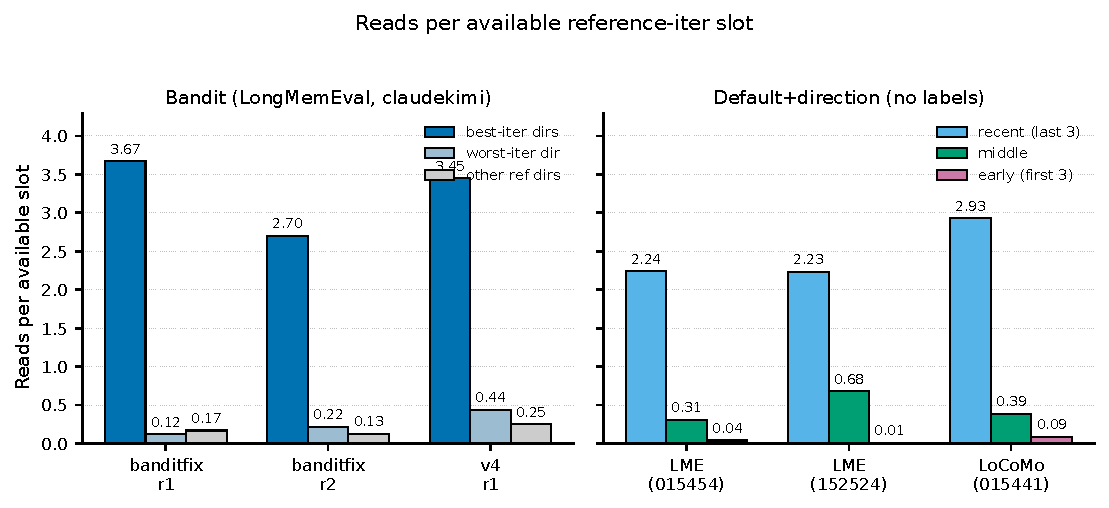
\includegraphics[width=\linewidth]{figures/read_concentration.pdf}
  \vspace{-6pt}
  \caption{Reference-iteration reads per available slot, averaged
  across three LongMemEval claudekimi runs per policy. Under
  bandit, best-tagged dirs receive $14$--$22\times$ more Read calls
  per slot than unmarked refs; the worst-tagged dir is read at the
  same rate as an unmarked ref. Under default, with no
  best/worst labels, the proposer falls back to a recency prior:
  the most recent three iters are read $30$--$220\times$ more often
  than the first three. The same fixed inspection budget is routed
  onto policy-labelled targets under \name and onto recency under
  default.}
  \label{fig:read_concentration}
\end{figure}

\textbf{(iv)~Progressive shows the same labelled-prior effect under a
post-hoc top-$k$ bucket scheme.}
Figure~\ref{fig:read_concentration} measures the labelled-prior effect
through the bandit's \texttt{best\_iterations} JSON state field.
Progressive does not write that field --- at \texttt{low} and
\texttt{medium} budget tiers it embeds the best/worst tag directly in
the prompt text (\S\ref{sec:iter_axis}) --- so the slot-normalised
statistic is bandit-only as written. To check whether progressive's
labelling redirects attention through the same channel, we apply a
bucket scheme that does not depend on the bandit JSON state: for every
Read tool call landing on \texttt{reference\_iterations/iter\_M/}, we
ask whether iter\_M was the current top-$1$ or top-$3$ by candidate
passrate at iteration $N$'s prompt-build time (the rank pool is
restricted to iters $< N$). Table~\ref{tab:top1_attention} aggregates
across two retained runs per (benchmark, policy) cell on the kimi
proposer (codex54 is excluded because its trace bucketing is
unavailable; cf.\ Figure~\ref{fig:read_concentration}).

\begin{table}[t]
\centering
\small
\caption{Where the proposer's reference-iteration Read calls land,
bucketed by post-hoc rank at prompt-build time. Each Read into
\texttt{reference\_iterations/iter\_M/} is classified by whether
iter\_M was the current top-$1$ / top-$3$ by passrate or among the
three most recent iters strictly $< N$. Top-$3$ and recent-$3$
buckets overlap by construction; \emph{other} is reads on iters in
neither bucket. Aggregated across r1+r2 per cell on the claudekimi
proposer (run IDs in
\texttt{scripts/measure\_top1\_attention.py}). Progressive's reads
land on the current top-$1$ iter at $\boldsymbol{+22}$--$\mathbf{26}$
percentage points higher share than \texttt{default} on both
benchmarks; LoCoMo additionally shows a $-23.1$\,pp drop in
recent-$3$ share, the labelled prior actively pulling reads off the
recency tail.}
\label{tab:top1_attention}
\begin{tabular}{@{}llrrrrr@{}}
\toprule
Benchmark & Policy & Total ref Reads & \% top-$1$ & \% top-$3$ & \% recent-$3$ & \% other \\
\midrule
\multirow{2}{*}{LongMemEval}
 & default            & $430$ & $52.1$ & $82.3$ & $60.2$ & $3.7$ \\
 & progressive       & $421$ & $\mathbf{77.7}$ & $\mathbf{87.6}$ & $55.6$ & $5.2$ \\
\midrule
\multirow{2}{*}{LoCoMo}
 & default            & $485$ & $31.1$ & $66.6$ & $\mathbf{59.4}$ & $8.7$ \\
 & progressive       & $422$ & $\mathbf{53.8}$ & $\mathbf{70.4}$ & $36.3$ & $15.6$ \\
\bottomrule
\end{tabular}
\end{table}

Progressive's reads land on the current top-$1$ iter at substantially
higher share than default's: $+25.6$\,pp
on LongMemEval ($77.7\%$ vs $52.1\%$) and $+22.7$\,pp on LoCoMo
($53.8\%$ vs $31.1\%$). This is the same labelled-prior effect that
the $14$--$22\times$ reads/slot statistic quantifies for bandit, only
observed through a bucket scheme that does not require the bandit JSON
state. Progressive is informative as a control because its
\texttt{best\_iterations} choice is just rank-by-current-passrate (no
UCB, no estimator), so the redirection cannot be attributed to a
sophisticated estimator --- the labelling itself is what moves the
proposer's reads. LoCoMo additionally shows a $-23.1$\,pp drop in
recent-$3$ share under progressive ($59.4\%\!\to\!36.3\%$), so on
LoCoMo the label does not just add attention onto top-$1$, it actively
pulls reads off the recency tail. The smaller LongMemEval recency drop
($-4.6$\,pp) is consistent with LongMemEval progressive runs spending
more iterations at the high budget tier, where progressive surfaces
no labels and behaves like \texttt{default} on the ref-iter
channel.

\textbf{Mechanism summary.}
Per-iteration read volume is roughly budget-invariant ($\sim$$20$
unique reads, $\sim$$1.3$ reread rate, $\sim$$57$ lines per
ref-read); escalating the budget does not buy more inspection
effort, only a different target distribution. Within that
distribution, \name's \texttt{best\_iterations} pointer captures a
$14$--$22\times$ share of the proposer's attention, and the same
labelled-prior effect surfaces in Progressive under a top-$k$ bucket
scheme (top-$1$ share $+22$--$26$\,pp over default,
Table~\ref{tab:top1_attention}). \name redirects the same fixed
inspection budget that default-family spends on a recency-biased tail
toward historically productive iteration and file targets. The
policy's labels, not the budget tier, drive the proposer's bounded
attention.
This redirection explains why the two axes should be read as
composable attention-routing strategies rather than independent
contributions. The iteration axis routes attention across prior
attempts, whereas the file axis routes the same limited read budget
across files within the exposed workspace.

\subsection{Ablation: how do the strategies interact?}
\label{sec:ablation}

The mechanism above identifies two levers---bounded attention
(cardinality control on which iters the proposer sees) and targeted
attention (best/worst-iter labels)---plus the file-axis hot pool that
routes reads within the exposed workspace. We use two ablations to
separate bounded historical exposure, labelled historical attention,
and file-level utility guidance.

\textbf{Iter-axis selection rules.}
We compare four cardinality-bounded variants against the
full-context baseline: \emph{Random@3} (sample three prior
iterations uniformly at random each propose), \emph{Recency@3}
(surface the three most recent iterations), \emph{Progressive}
(best/worst-tagged budget state machine), and \emph{\name}
(adds file-axis hot pool on top of Progressive). All four keep
identical source-snapshot, summary, and file-tree exposure; only
the iter-axis selection rule changes. We set $k\!=\!3$ to match the
median ref-iter exposure of Progressive's medium tier.

\textbf{Force-budget runs.}
To separate the contribution of the budget tier itself from the
contribution of policy labels, we additionally pin every iteration
to a single tier. \emph{Bandit force=low} freezes the budget at
\texttt{low} (no ref-iter dirs surfaced for bandit); \emph{Bandit
force=high} freezes it at \texttt{high} (full ref-iter exposure).
Six claudekimi runs, 30 iterations each.

Table~\ref{tab:ablation} reports both ablations alongside default
and the main policies. Iter-axis ablation rows are run on
LoCoMo / codex54 (the only cell with retained Random@$3$ /
Recency@$3$ runs); force-budget rows are claudekimi train passrate.

\begin{table}[t]
\centering
\small
\caption{Ablation. \emph{Top block:} iter-axis selection-rule
ablation on LoCoMo / codex54 ($n\!=\!3$ retained runs per row).
\emph{Bottom block:} force-budget runs on claudekimi memory
benchmarks; \emph{train best} is the cell-best train passrate
under the forced tier. \emph{ref share} is reference-iter reads
as a fraction of all Read calls; \emph{best/prop} is reads of
\texttt{best\_iterations}-tagged dirs.}
\label{tab:ablation}
\begin{tabular}{@{}llrrrrrr@{}}
\toprule
Cell / setting & Policy & test or train & best test & total/prop & ref/prop & ref share & best/prop \\
\midrule
\multicolumn{8}{l}{\textit{Iter-axis selection ablation (LoCoMo / codex54, test)}} \\
 & default-family   & $0.331 \pm 0.013$       & $0.340$        & $3.42$M & --- & --- & --- \\
 & Random@$3$       & $0.360 \pm 0.027$       & $0.391$        & $2.66$M & --- & --- & --- \\
 & Recency@$3$      & $0.346 \pm 0.035$       & $0.386$        & $2.72$M & --- & --- & --- \\
 & Progressive      & $\mathbf{0.374 \pm 0.014}$ & $\mathbf{0.388}$ & $2.46$M & --- & --- & --- \\
 & \name (iter+file) & $0.355 \pm 0.027$      & $0.387$        & $\mathbf{2.14}$\textbf{M} & --- & --- & --- \\
\midrule
\multicolumn{8}{l}{\textit{Force-budget ablation (claudekimi memory, train)}} \\
LoCoMo & bandit force=high   & train $\mathbf{0.4000}$ & ---  & $4.21$M & $9.58$  & $36.4\%$ & $\mathbf{7.84}$ \\
LoCoMo & bandit force=low    & train $0.3875$ & ---  & $2.79$M & $\mathbf{0.02}$ & $\mathbf{0.1\%}$ & $\mathbf{0.00}$ \\
LongMemEval & bandit force=high & train $0.5800$ & --- & $3.73$M & $9.58$  & $36.4\%$ & $7.84$ \\
LongMemEval & bandit force=low  & train $\mathbf{0.6300}$ & --- & $2.83$M & $\mathbf{0.02}$ & $\mathbf{0.1\%}$ & $0.00$ \\
\bottomrule
\end{tabular}
\end{table}

\textbf{Bounded attention beats full context, and the iter-axis
selection rule is not the primary driver.}
All four cardinality-bounded variants score above default-family on
test passrate ($+1.5$ to $+4.3$\,pp) and are cheaper on per-propose
tokens ($-22\%$ to $-37\%$). Random@$3$ and Recency@$3$ both
exceed default by $+1.5$ to $+2.9$\,pp despite using uninformative
selection rules. The four bounded variants also sit within
$\sim$$3$\,pp of each other on test, well inside cell std. Two
structural properties of our setup explain why the iter-axis
\emph{targeting} rule matters less than expected: (a)~the proposer
rebuilds each candidate from the same baseline harness rather than
incrementally patching the current best, so even an uninformative
iter sample is recoverable as long as the proposer is not asked to
digest the full history; and (b)~Section~\ref{sec:mechanism}'s
read-decomposition shows summary reads holding tier-invariant at
$\sim$$5\!-\!6$ per propose---cumulative summaries form a
persistent cross-session context channel that any iter-selection
rule benefits from. \name remains the cost leader at $2.14$M
total/propose, $\sim$$20\%$ cheaper than Random@$3$ and Recency@$3$
at comparable test passrate; the file-axis is what pulls \name to
a Pareto-favorable point under matched cardinality.

\textbf{Strong file-level signal can compensate for a closed
reference-iteration channel.}
Bandit force=low almost completely removes the reference-iteration
channel ($0.02$ ref reads/propose, zero best-iter reads, zero ref
lines) versus $9.58$ ref reads and $7.84$ best-iter reads at
force=high---the $36.4\% \!\to\! 0.1\%$ collapse is the
controlled-ablation evidence that the budget tier opens the
reference-history channel. Despite this complete channel removal,
LongMemEval bandit force=low reaches train $0.6300$, the highest
train passrate among retained LongMemEval bandit runs (above
force=high's $0.5800$). Thus, the LongMemEval setting contains enough
file-level signal for the UCB hot pool to carry the search when the
reference channel is closed. On LoCoMo,
force=low reaches train $0.3875$ versus force=high's
$0.4000$, a small drop, indicating that explicit reference-history
access adds value on smaller candidate codebases where historical
labels provide concrete prescription. The Pareto trade is therefore
benchmark-conditional, not absolute: file-axis curation can capture
most of the gain when file-pool signal is rich, while the iter-axis ref
channel acts as additional guidance when historical examples are
especially informative.
